\chapter{Grundlagen}

In diesem Kapitel werden die für die Entwicklung benötigten verwendeten technischen Grundlagen erläutert.

\section{REST}

REST ist eine Abkürzung für Representational State Transfer und wurde von Roy Fielding in seiner Dissertation aus dem Jahr 2000 \cite{rest} definiert. Es handelt sich hierbei um eine Auflistung von Eigenschaften und Anforderungen, welche durch eine REST-API erfüllt werden sollen. REST-APIs werden für viele Dienste des Internets meist unsichtbar für die Anwender für die Kommunikation zwischen informationstechnischen Systemen verwendet. In der englischen Sprache wird häufig der Begriff "RESTful" für Ressourcen verwendet, welche die REST-Prinzipien anwenden.

\section{Telegram Messenger}

Der Dienst Telegram bietet seinen Nutzern eine Möglichkeit um kostenlos miteinander u.A. über Apps für die Mobilbetriebssysteme Android und iOS zu kommunizieren. Telegram hatte nach nach eigenen Angaben weltweit im Juni 2022 erstmals über 700 Millionen monatliche Nutzer und befand sich unter den fünf Apps mit den höchsten Downloadzahlen \cite{telegram-700-million}. Der Dienst stellt damit eine beliebte Alternative zu anderen Messengern wie WhatsApp oder Signal dar. Ein Alleinstellungsmerkmal von Telegram sind Bots und die dazugehörige API.

Der Begriff Bot stammt von dem englischen Begriff robot ab und bezeichnet eine Computersoftware, welche einfache und wiederkehrende Aufgaben selbstständig erledigt. Bots werden heutzutage an vielen Stellen beim Kontakt von Menschen und informationstechnischen Systemen eingesetzt, beispielsweise in Telefonwarteschleifen oder in Webshops in Form von virtuellen Beratern für den Verkauf oder den Service. Der Telegram Messenger bietet Softwareentwicklern die Möglichkeit, mittels einer HTTP-API einen Bot auf vielfältige Weise an eigene Software anzubinden. Der Bot agiert Benutzern auf der Telegram Plattform gegenüber wie ein normaler Verbindungspartner mit dem Unterschied, dass dieser zuerst mit einer Initialnachricht (\lstinline{/start}) vom Benutzer aktiviert werden muss. So wird verhindert, dass  Benutzer ohne Zustimmung kontaktiert werden können. Bots können ebenfalls zu Gruppen hinzugefügt werden. Dem Entwickler stehen zahlreiche und ausführlich dokumentierte API-Funktionen \cite{telegram-bot-available-methods} zur Verfügung, sodass die vom Bot ausgehende Kommunikation nicht auf Textnachrichten limitiert ist. Bots stehen u.A. folgende Möglichkeiten zur Verfügung:

\begin{itemize}
\item Senden und Empfangen von Audio-, Bild- und Videodateien
\item Senden und Empfangen von Sprachnachrichten
\item Senden und Empfangen von Standorten
\item Eröffnen von Abfragen
\item Abfrage von Informationen der aktiven Kommunikationspartner: Profilbild, Name, Zeitpunkt der letzten Erreichbarkeit (sofern vom Benutzer freigegeben)
\item Gruppenadministration: Setzen und Entfernen von MOTD-Nachrichten
\item Vereinfachte Bedienung durch vom Entwickler definierte Antwortmöglichkeiten, welche durch den Anwender direkt mittels Buttons gewählt werden können
\end{itemize}

Aufgrund der weitreichenden Möglichkeiten, der kostenlosen Benutzbarkeit und der auch für frequentierte Applikationen ausreichend dimensionierten Durchsatzratenbegrenzung \cite{telegram-bot-rate-limit} steht eine Vielzahl von Bots für die Benutzer der Plattform zur Verfügung. Als Beispiele seien genannt der Bot "WDR aktuell" <\lstinline{@WDRaktuell_bot}> für den Abruf von regionalen Informationen in Nordrhein-Westfalen, der von Google angebotene und daher als "verifiziert" markierte "Gmail Bot" <\lstinline{@GmailBot}> für den Nachrichtenabruf und das Senden von Antworten für Gmail sowie der Bot IFTTT <\lstinline{@IFTTT}>, welcher ebenfalls als "verifiziert" markiert wurde, da dieser vom Entwickler des Dienstes für Automatisierung und Verknüpfungen von Webanwendungen IFTTT ("if this then that") bereitgestellt wurde.

\begin{figure}[hb!]
\centering
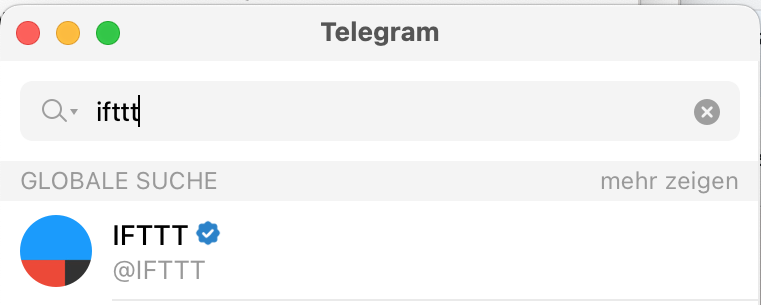
\includegraphics[scale=0.5]{verified_ifttt_bot}
\caption{Verifizierter IFTTT-Bot in der Suche von Telegram für macOS.}
\label{abb_einstein}
\end{figure}

\subsection{Beziehen von Aktualisierungen von der Telegram API}

Laut der technischen Dokumentation der Telegram API \cite{telegram-getting-updates} stehen zwei Möglichkeiten zur Verfügung, um Aktualisierungen zu erhalten: \lstinline{long-polling} der API-Methode \lstinline{getUpdates()} oder die Verwendung eines \lstinline{webhooks}. Die beiden Möglichkeiten verwenden unterschiedliche Konzepte und bieten damit verschiedene Vor- und Nachteile: im Fachbereich der Informatik steht der Begriff \lstinline{polling} für eine dauerhafte wiederkehrende Abfrage von Informationen bei einem Dienst. Diese Technik beansprucht viel CPU-Zeit eines Systems und wird aufgrund des geringen Gegenwerts der meist leer ausgehenden Abfragen als teuer bezeichnet. \lstinline{long-polling} beschreibt eine Technik, bei welcher der Client einer HTTP-Abfrage einen verlängerten Zeitraum bis zum Erhalt der Antwort vom Server akzeptiert, ohne die Abfrage aufgrund einer Zeitüberschreitung abzubrechen. Die Länge des Zeitraums ist variabel. \lstinline{long-polling} bietet damit gegenüber dem klassischen \lstinline{polling} den Vorteil, dass die benötigte Rechenzeit durch die verlängerten Abfragezeiträume stark reduziert wird. Die Software- und Betriebssystementwicklung bietet eine Technik, um die Verwendung von teurem \lstinline{polling} zu umgehen: die Verwendung von \lstinline{interrupts} oder \lstinline{callbacks} (zu deutsch "Rückruf"). Hierbei erhält der Absender der Anfrage eine Rückmeldung, sobald die Antwort vorliegt. Der Vorteil dieser Technik ist, dass nach dem Absenden der Anfrage keine CPU-Zeit seitens des Absenders notwendig ist. Es muss jedoch eine Möglichkeit vorhanden sein, den Absender im Falle einer eingehenden Antwort zum Vorgang zurückzuführen, sodass die weitere Bearbeitung möglich wird. Im Falle der Anbindung der Telegram API übernimmt dies der \lstinline{webhook}. Der \lstinline{webhook} muss (durch die Telegram-API) öffentlich aus dem Internet erreichbar und durch den Verwalter des Bots im Vorhinein durch eine entsprechenden URL definiert worden sein. Wird eine Nachricht an den Bot gesendet, prüft die Telegram-API, intern, ob Definitionen für webhooks vorliegen. Im positiven Fall sendet die Telegram API eine HTTP-Anfrage an die URL des webhooks mit den Details zur eingegangenen Nachricht. Nach Erhalt der Anfrage durch den webhook muss dieser die Daten zur verarbeitenden Software zurückführen und die weitere Bearbeitung auslösen.